


\section{Review of PubChem Assay 1851}
  

PubChem BioAssay 1851 contains data for inhibition of five major CYP isoforms (1A2, 2C9, 2C19, 2D6 and 3A4) by 17,143 chemical compounds. \cite{Veith2009} The the tested compounds were all drugs or drug-like compounds. The chemical space revealed that the majority of compounds had molecular weight below 500 daltons and logP below 5. \cite{Lapins2013}

The assay used low low-fluorescence substrates, which are converted to more-fluorescent metabolites. The progression of the reaction is measured by an increase in fluorescence intensity during CYP isozyme metabolism of the substrate. Inhibitors of a particular CYP reduce the rate of metabolism of the substrate and this results in a decreased fluorescence signal. \cite{Zlokarnik2005}

The most recent technology developed for CYP inhibition is based on substrates that release luciferin as the metabolite. This is a coupled assay system in which addition of luciferase and ATP converts the freed luciferin to des-carboxyluciferin with light emission. The format is similar to fluoresence methods, and all that is required is addition-only manipulations and luminescence plate readers. \cite{Zlokarnik2005} The assay obtained lumiescence readings at a range of compound concentrations and then determined activity parameters using the Hill equation.


%Inorganic compounds, non-covalent inhibitors and compound mixtures were removed from the dataset, leaving 16,359 compounds. \cite{Lapins2013}

In the dataset, compounds are classified as active or inactive inhibitors for each CYP with an activity cutoff set to AC50 = 10uM (AC50, “activity concentration 50”, refers to the concentration that is required to elicit half-maximal effect). However, in cases where the dose-response curve for a compound showed poor fit or the inhibition efficacy was below 60\%, the assay results were regarded as inconclusive. \cite{Lapins2013}

Compounds were characterized by their Activity Score and regarded as inhibitors if their activity score ranged between 40 and 100. PubChem Acitivity Score is assigned based on AC50 value, which was combined with a confidence measure. Combining measures for completeness of a dose-response curve and efficacy of inhibition, resulted in the Activity Score, where a larger value indicates higher inhibitory activity and/or higher confidence in inhibitory assay result. Compounds with an activity score equal to zero are considered as non-inhibitors while compounds with activity scores above 0 and up to 40 are considered inconclusive. \cite{Lapins2013}

The data from Pubchem Assay 1851 is available for download from the NIH through the PubChem website. The interface changes from time to time, but I downloaded two files which comprised the entire dataset for the experiment. The first file, a structures file, contained the structural information encoded in the simplified molecular-input line-entry system (SMILES) format for each tested compound with corresponding Structure ID (SID) and Compound ID (CID) as assigned by NCBI. Another file, also organized by SID and CID, contained all of the luminescent responses from the high-throughput screen and the fitted parameters which are then summarized by the activity score. 

\begin{figure}[!htbp]
  \caption{Supervised Learning Scheme for Clasification}
  \centering
  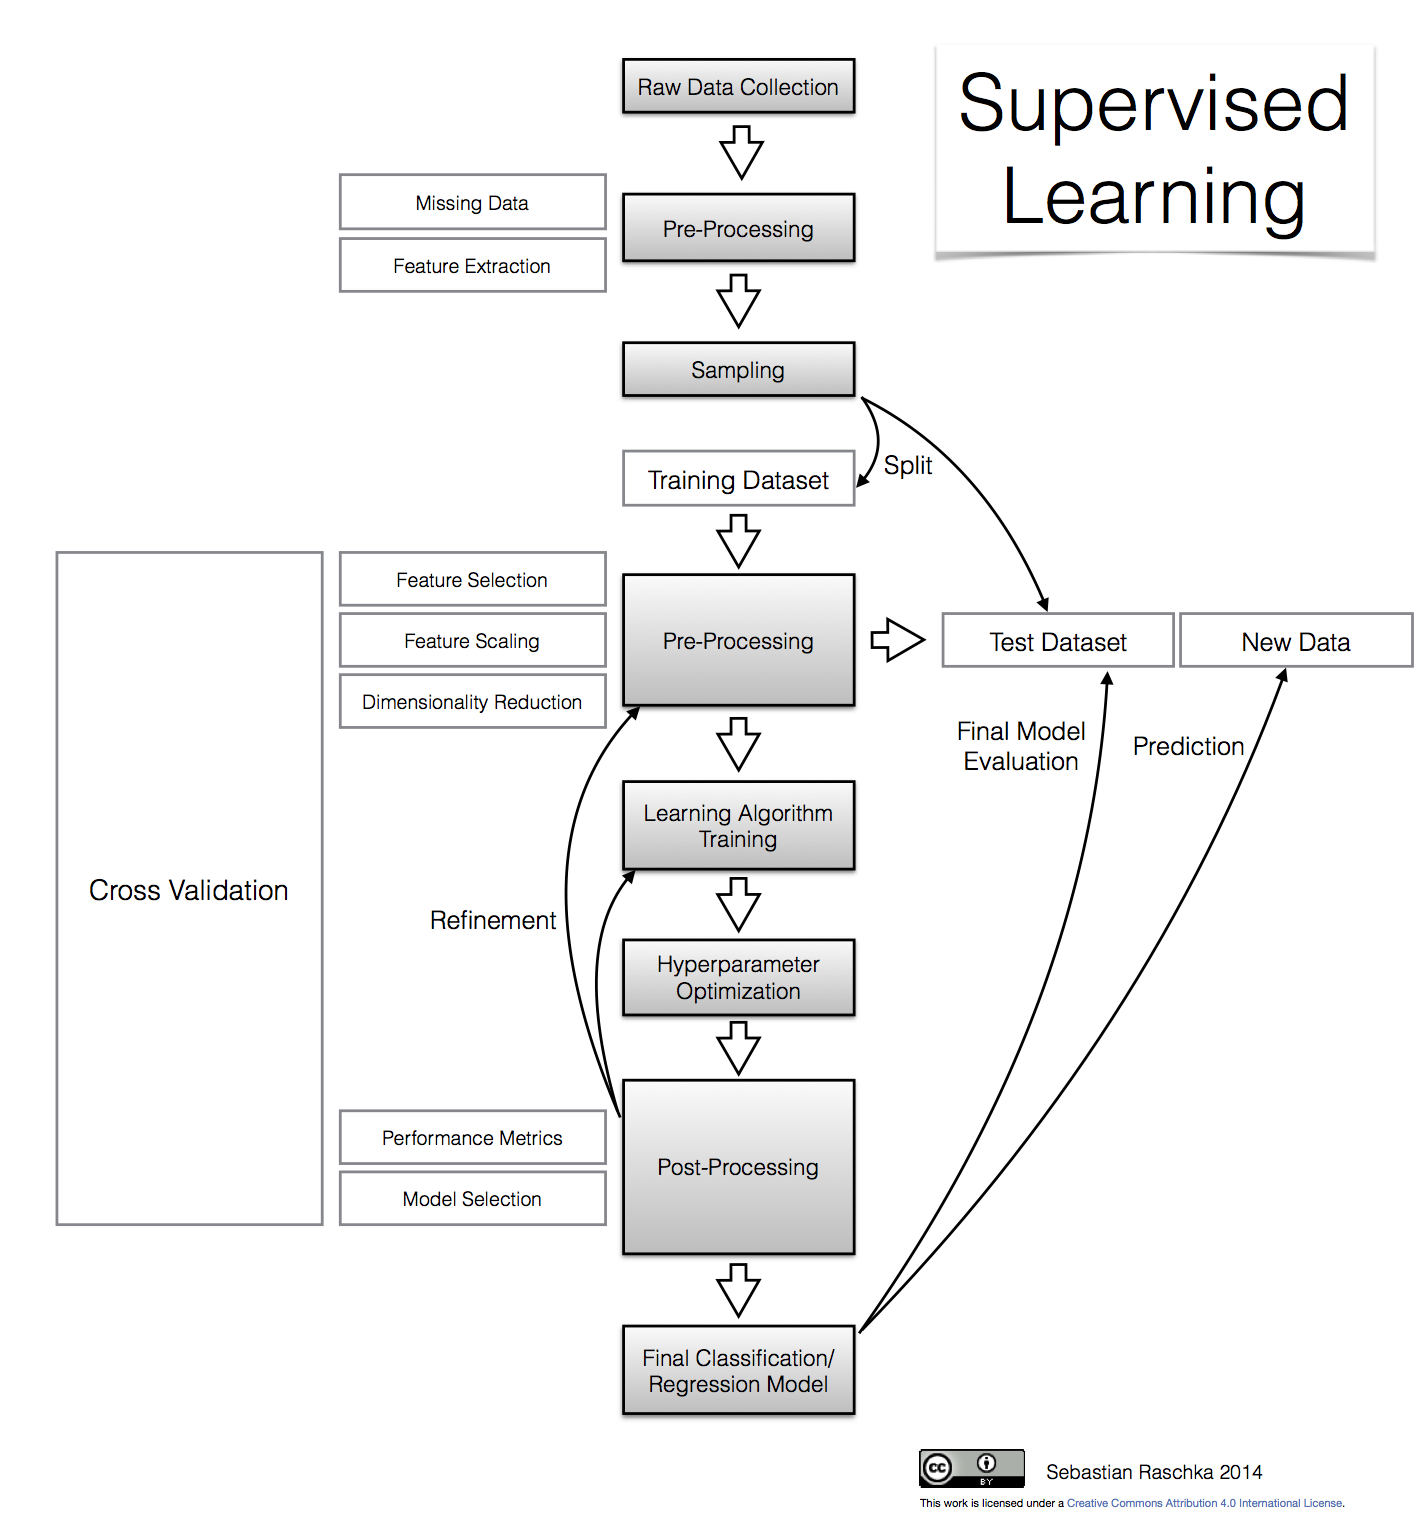
\includegraphics[width=1\textwidth]{../img/supervised_learning_flowchart.png}
\end{figure}


\section{Data Set Preparation and Molecular Descriptor Generation }

Both data files from Bioassy 1851 were downloaded as comma separated value (.csv) files and merged together based on the SID column using functions from Python's pandas library, which is made for handling, manipulating and reshaping structured data.

The preliminary steps of data preprocessing typically requires data cleaning as raw data often contain anomalies, errors, or inconsistencies such as missing data, incomplete data, and invalid character values which may cause trouble in data analysis if left untreated. It is more complicated when data are collated from many formats that require harmonization and redundancy elimination. \cite{Nantasenamat2009} In this case, minimal preprocessing was required due to the polished nature of the source files.


\begin{figure}[h,t]
  \caption{Data download and preparation}
  \centering
   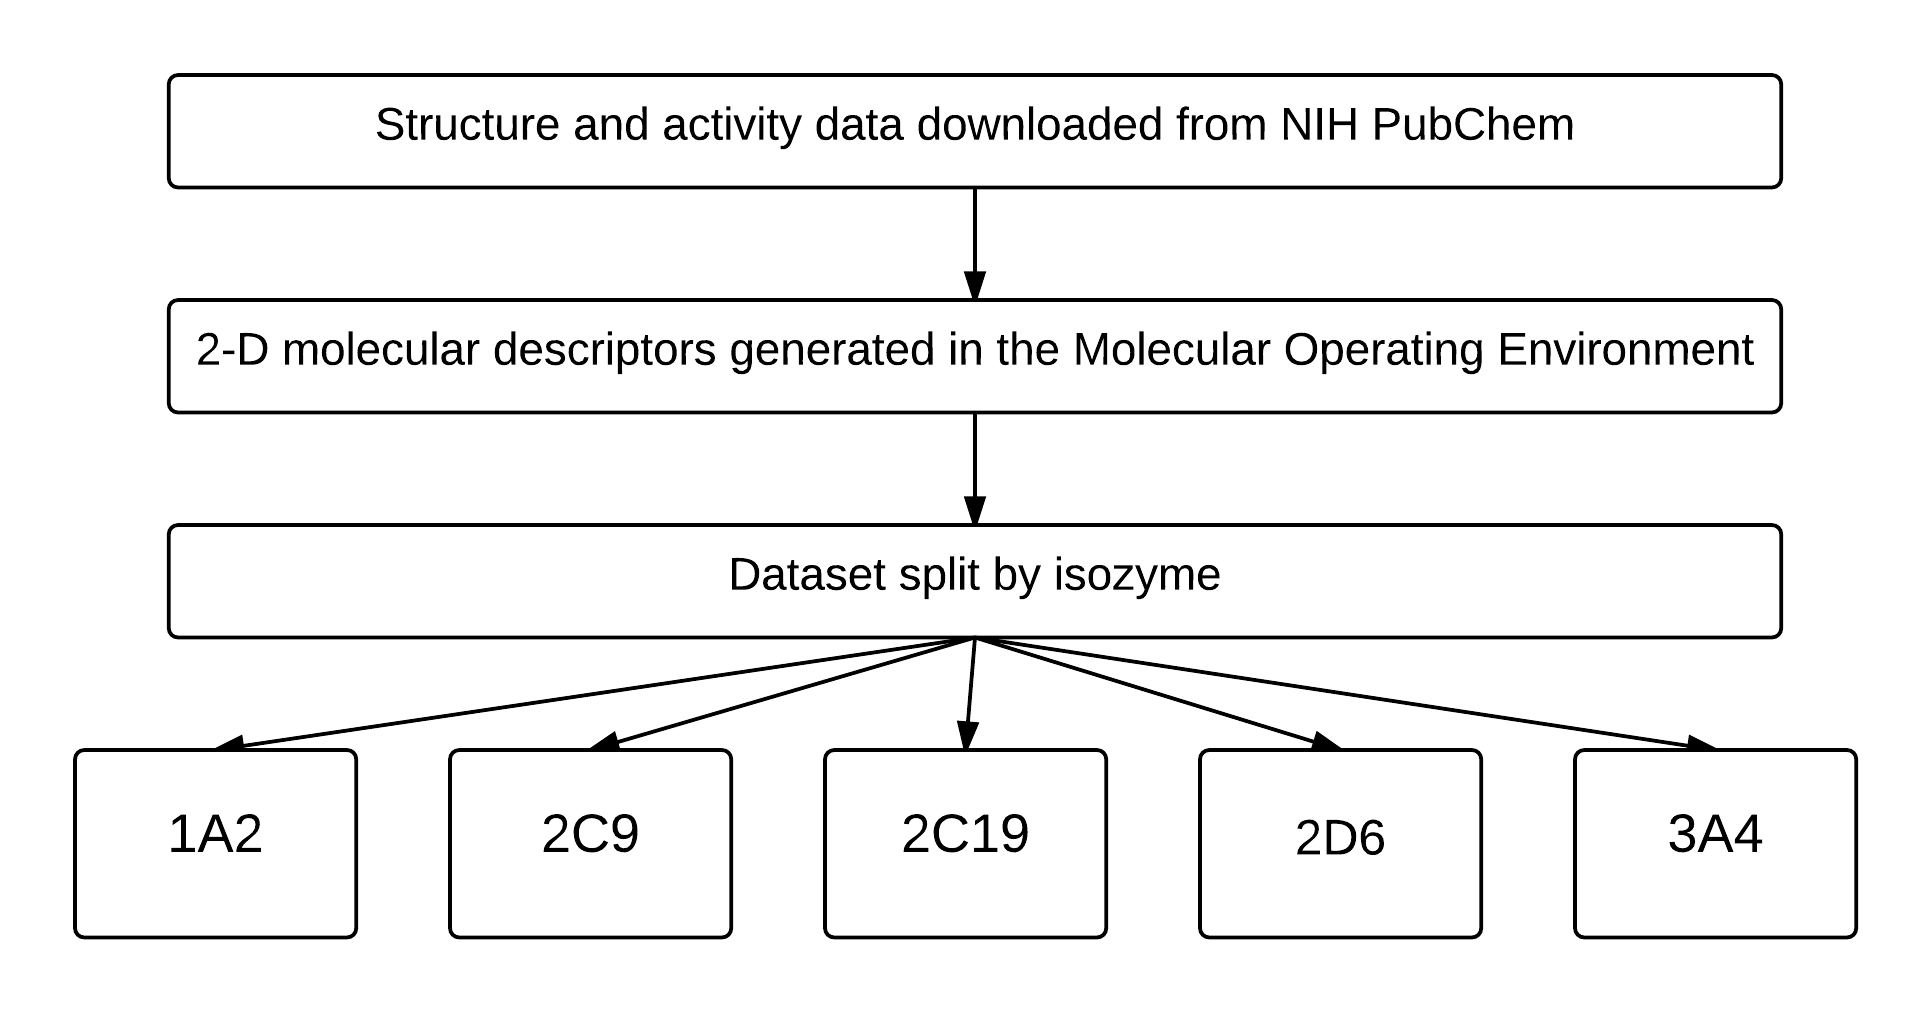
\includegraphics[width=1\textwidth]{../img/Dataset_prep.png}
\end{figure}


\subsubsection{Molecular Descriptor Generation}
First the merged file was loaded into a database in the Molecular Operating Environment. MOE functionality was used to obtain the washed configuration of compounds by removing the salts and finding an energy-minimized conformation. MOE was then used to calculate descriptors based on the molecular structures. The entire suite of MOE 2-D descriptors was selected for descriptor generation, resulting in 186 additional columns of nominal, ordinal and continuous vales appended to the database. The resulting master file was saved in .csv format.

The dataset was then split by isozyme into 5 separate files that each contained only the SID, the Activity Score, and the 186 MOE 2-D descriptors using a script in the Python programming language.

For each isozyme, the number of active inhibitors was far outnumbered by the number of inactive inhibitors. The data file for each isozyme was subjected to a Python script that separated the inactives from actives. Then the order of the inactives was randomly shuffled and the column trimmed to the length of the activity column, thereby balancing the number of inactives and actives as required by some of the later statistical analyses. 

\begin{figure}[h,t]
  \caption{Isozyme data set preparation}
  \centering
   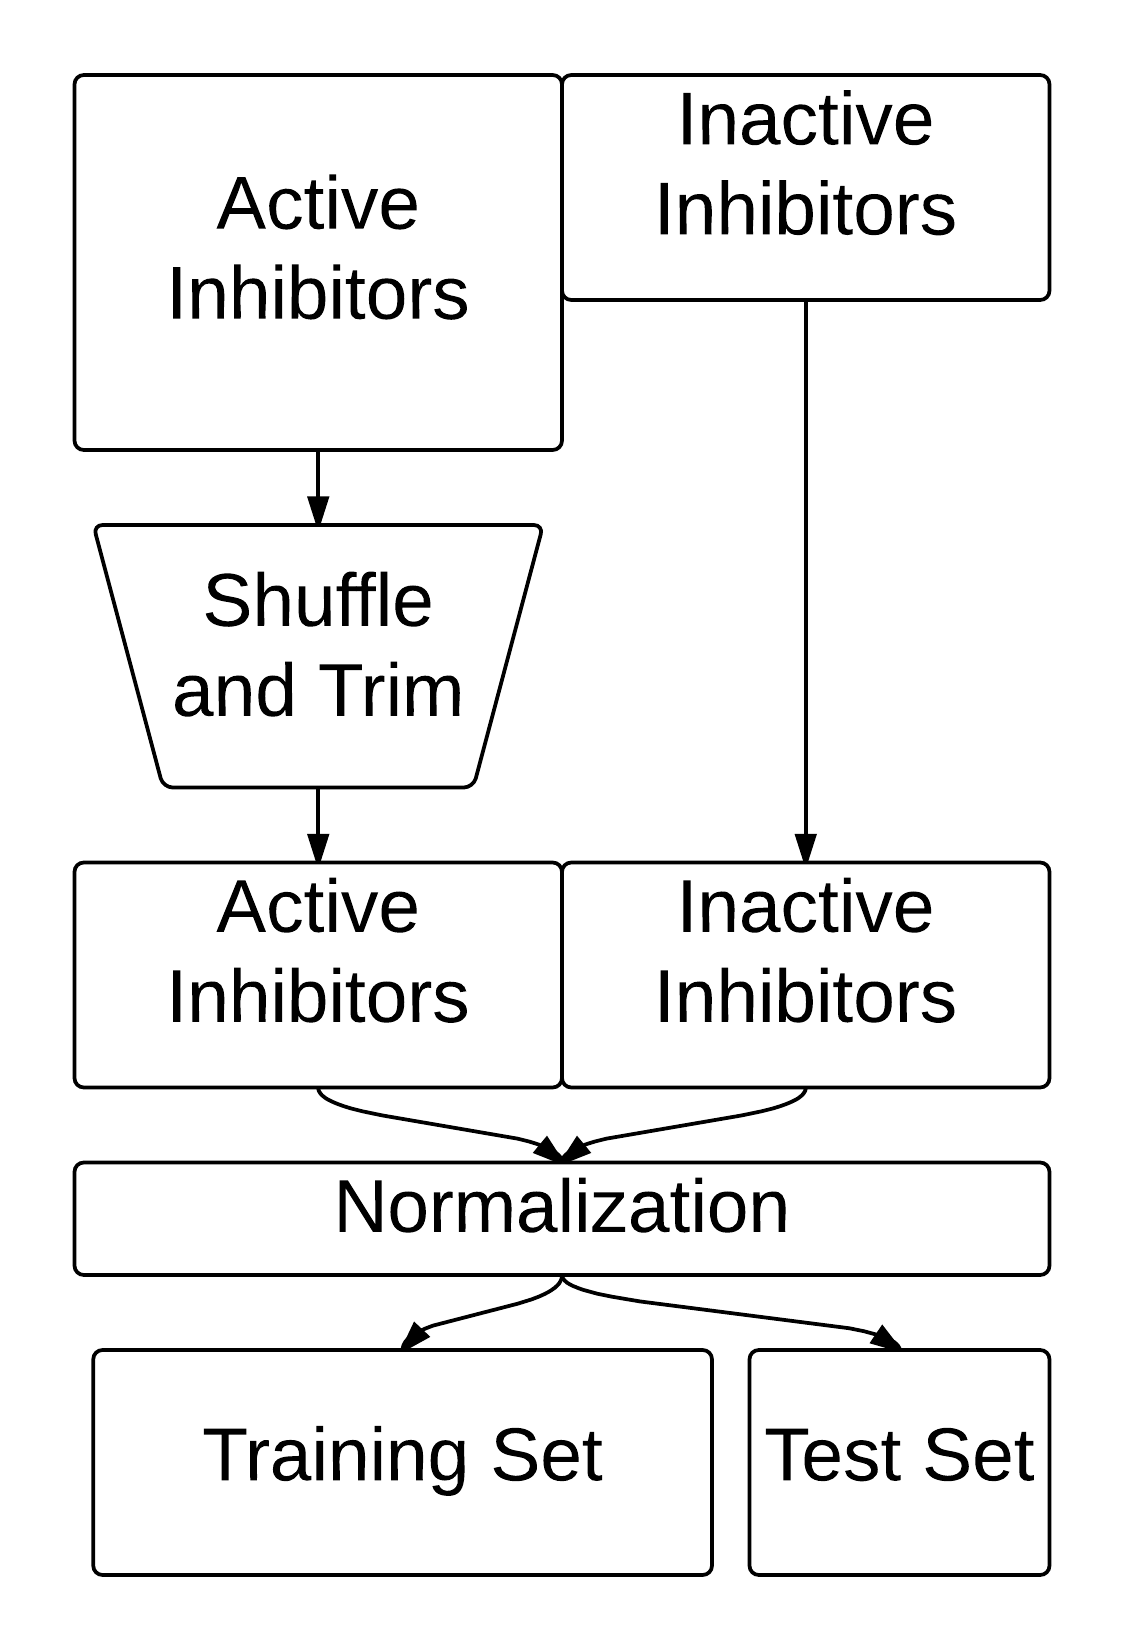
\includegraphics[width=1\textwidth]{../img/Isozyme_Data_Prep.png}
\end{figure}

Next the script randomly shuffled the balanced datasets and split them into a training set and a test set. The training set held 80\% of the original values and the test set held 20\% of the original values. The split was not based on activity score. The ratio of active/inactive in each split was inspected to check if they were still acceptably balanced.

For each use of randomness in computation, a seed number was set for the random number generator to ensure reproducible results.  

The balanced and split datasets are saved to Figshare.com for permanent, free and open access. (http://dx.doi.org/10.6084/m9.figshare.1181846 and http://dx.doi.org/10.6084/m9.figshare.1066108) All subsequent analyses use these same splits for comparability.

\section{Feature selection}

Typically data sets often contain redundant or noisy variables which make it more difficult for learning algorithms to discern meaningful patterns from the input. Such multicollinearity of the variables can either be used or treated if necessary to reduce computational resources required for model construction. \cite{Nantasenamat2009}

There existed a great deal of variability in the range and distribution of each variable in the data set. This can pose problems for algorithms using distance measurements in the learning step. These situations are handled by applying statistical techniques such as min-max normalization or z-score standardiation. 

In min-max normalization, the minimum and maximum value of each variable is adjusted to a uniform range between 0 and 1 according to the following equation: $ X_{norm} = \frac{X - X_{min}}{X_{max} - X_{min}}  $ In z-score standardization, essentially the variable of interest is subjected to statistical operation to achieve mean center and unit variance according to the following formula: $ z = \frac{x - \mu}{\sigma}  $ \cite{Nantasenamat2009}

In situations where the data does not have a Gaussian (normal) distribution, simple mathematical functions can be applied to achieve normality or symmetry in the data distribution. A commonly used approach is to apply logarithmic transformation on the the variable of interest in order to achieve distribution approaching normality. This is typically performed on dependent variables such as the modeled biological/chemical properties of interest whereby IC50 may be transformed to logIC50 or -logIC50. Practically, such mathematical operation is applied to each individual value of a given variable of interest. \cite{Nantasenamat2009}

\section{Modeling - Mapping Descriptors to Activity Data}

At this point a complete dataset is assembled for each isozyme that is balanced for the number of active and inactive inhibitors, and that dataset has been further subdivided into a traing set and a test set. The following section describes the different methods of feature selection, normalization and classification algorithms used in this study.

\begin{figure}[h,t]
  \caption{Supervised Classification Model Training and Validation}
  \centering
   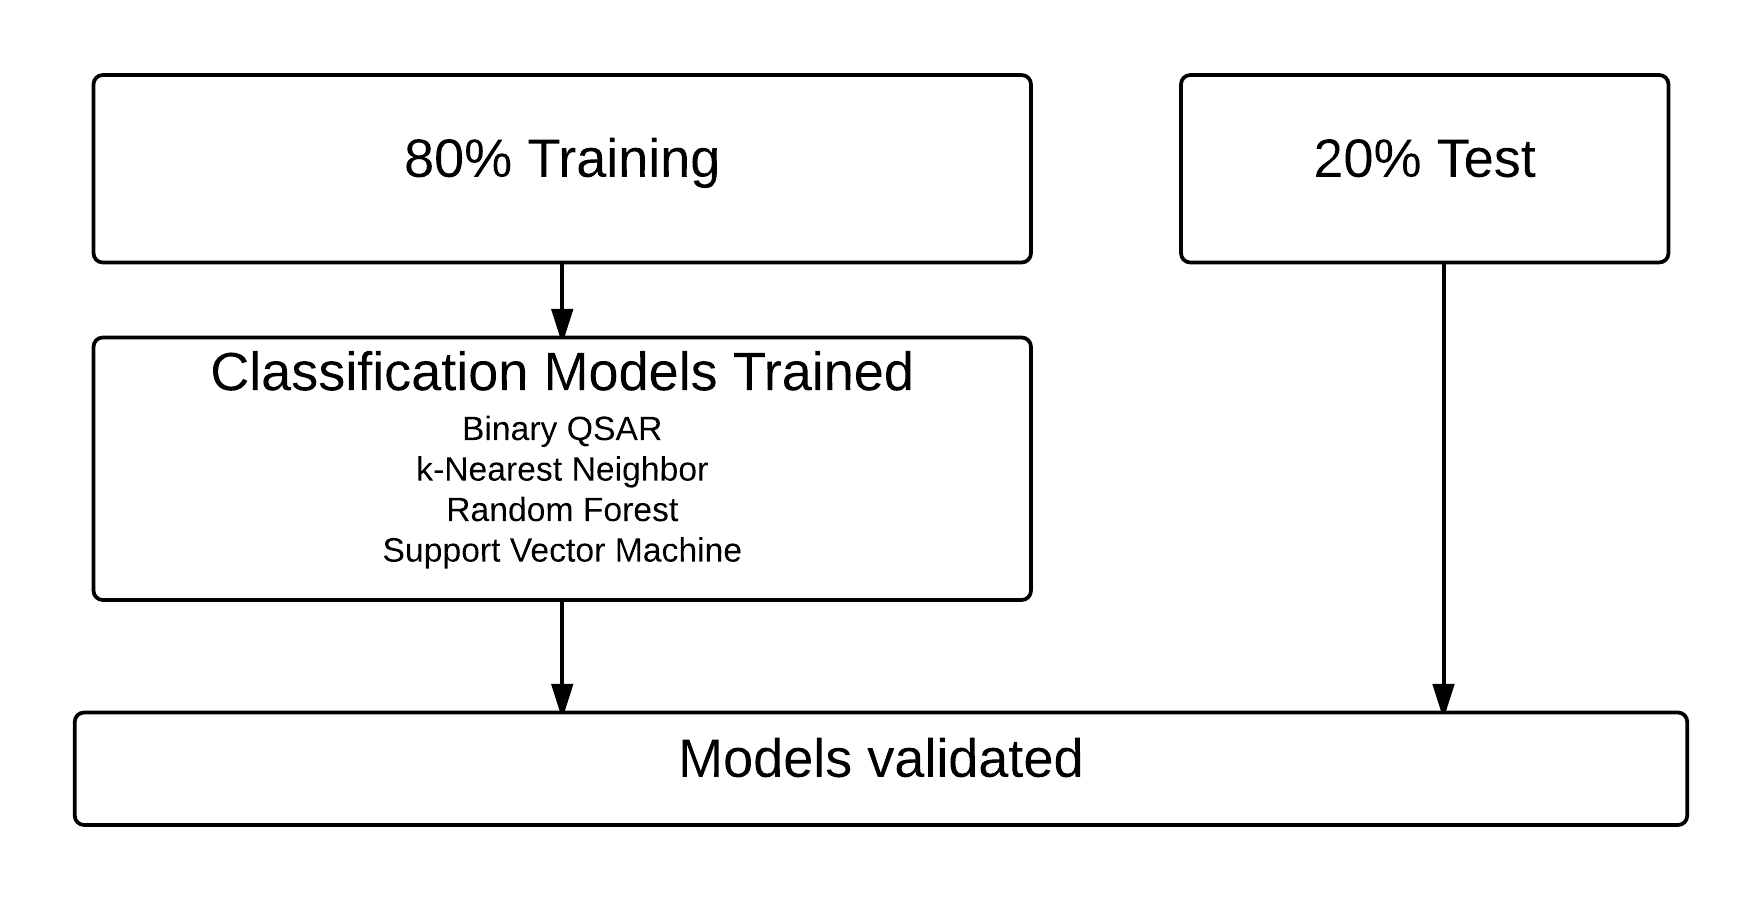
\includegraphics[width=1\textwidth]{../img/Model_validation.png}
\end{figure}

\subsection{Binary QSAR in the Molecular Operating Environment}
PLS regression is a qunatitative method available in the Molecular Operating Environment that has shown poor predictive accuracy with this dataset as demonstrated by previous attempts in Dr. Zheng's lab.

The Binary QSAR approach outlined by Labute \cite{Labute1999} and included in the 2011 version of MOE, takes a Bayesian and probabilistic approach to classification of activity after reducing all the descriptors to principal components.

To carry out this analysis, first the training data was loaded into MOE and used a menu driven interface to initiate the Binary QSAR methods. A threshold value of 39 was selected; all activity values 40 and above will be considered active and all values 39 and below are considered inactive. The smoothing parameter was left at the default value of 0.25. MOE automatically performs principal component analysis on high-dimensional datasets before Binary QSAR and there was no way to use the fuul suite of molecular descriptors.

For each isozyme a number of models were built, each using a different number of principal components.  Each principal component is orthogonal and uncorrelated to the rest, and each one captures a portion of the total variance inherent in the dataset. The assumption is that inclusion of more principal components leads to more of the variance being accounted for in a classification decision. However, since each principal component is a linear combination of all the variables, the benefits of dimensionality reduction comes at the cost of interpretability.  For exploratory purposes, models with 2, 5, 10, 15, 20, 30, and 44 principal components were constructed. 

MOE models were written to .fit files and the model report saved as a .txt file.

\subsection{$\kappa$-Nearest Neighbor ($\kappa$NN}
The kNN algorithm predicts the class of a test set object based on the class membership of its $\kappa$ most similar training set objects. \cite{Lapins2013}

\subsection{Random Forest (RF)}
Random Forest is a classifier that consists of multiple decision trees. A decision tree is made of nodes and branches. At each node the dataset is split based on the value of some attribute that is selected so that the instances of different classes are predominately moved to different branches. Classification starts at the root node and is performed by passing the instances along the tree to leaf nodes. \cite{Lapins2013}

To introduce diversity between the trees of a random forest, a small subset of all attributes is randomly selected to take decisions at each node of each tree. The classification decision is performed by considering results of all trees by majority vote. The optimal size of the forest and the number of attributes to consider at each node were found by performing five-fold cross-validation. \cite{Lapins2013}

\subsection{Support Vector Machines (SVM)}
SVM is a machine learning technique for classification or regression that uses linear or non-linear kernel-functions to project the data into a high-dimensional feature space. \cite{Lapins2013}

%Correlation is performed in this hyperspace based on the structural risk minimization principle i.e., aiming to increase the generalization ability of a model. \cite{Lapins2013}

They applied the commonly used Gaussian radial basis function kernel optimal gamma (width of the kernel function) and error penalty parameter C were found after performing grid search on five­fold cross validation. \cite{Lapins2013}


\section{Model Evaluation and Validation}

The building blocks of a successful QSAR model are the accuracy of the input data, selection of appropriate descriptors and statistical tools, and most importantly validation of the developed model. Validation is the process where reliability and relevance of a procedure are established for a predetermined purpose. For QSAR models validation should target robustness, predicition performances and applicability domain (AD) of the models. \cite{Lapins2013}

Statistical evaluation in QSAR modeling is essential to validate the model as well as to evaluate its predictive performance. The predictive performance of a data set can be assessed by dividing it into a training set and a testing set. The training set is used for constructing a model and then the predictive performance of that model is evaluated on the testing set. Internal performance is typically assessed from the predictive performance of the training set while external performance can be assessed from the predictive performance of the independent test set that has never been seen by the training model. A commonly used approach for internal validation is known as N-fold cross-validation where a data set is partitioned into N number of folds. For example, in a 5-fold cross-validation 1 fold is left out as a testing set while the remaining 9 folds are used as the training set for model construction and then validated with that fold left out. In situations where the number of samples is limited, leave-one-out cross-validation is the preferred approach. In that case, the number of folds is equal to the number of samples present in the data set. \cite{Nantasenamat2009}

%Some standard measures of performance used for QSAR models are sensitivity, specificity, positive predictivity, negative predictivity and concordance. Additional measures such as the Matthews coefficient can be used as a single metric for comparing one model to another while correcting for bias. Because most stat models can be modified to have greater specificity vs sensitivity (or vice versa) by adjusting the training set or applying predictive filters, the Matthews coefficient can be used to determine when the modification is so extreme that it leads to overall degradation of the models’ performance.\cite{Kruhlak2012}

%Statistical parameters - Pearson's correlation coefficient (r) is a commonly used parameter to describe the degree of association between two variables of interest. Calculated r values have values between -1 and +1 which indicate direct (positive) and indirect (negative) correlation. For describing the relative predictive performance of a QSAR model, r is used to measure the correlation between experimental (x) and predicted (y) values of interest in order to observe the variability that exists between variables. This is calculated according to the following equation: ...

%Root mean squared error (RMS) is another commonly used parameter for assessing the relative error of the QSAR model. RMS is computed according to the following formula: ...

%F-test -- The statistical significance of QSAR models are typically assessed by performing an ANOVA and observing the calculated F values, which is essentially the ratio between the explained and unexplained variance. Comparison between multiple QSAR models can be performed when all models have the same number of degrees of freedom meaning that the same sets of compounds and descriptors are used. Each model yields a calculated F value and the best performing model is identified as those bearing the highest value.\cite{Nantasenamat2009}

%Degrees of freedom take into consideration the number of compounds and the number of independent variables that are present in the data set. This can be calculated using the equation n - k - 1 where n = \# of compounds k = \# of descriptors. The higher the value, the more reliable the QSAR model is. \cite{Nantasenamat2009}

%Mathematically speaking, an outlier is essentially a data point which has a high standard residual in absolute value when compared to other samples in the data set. A commonly used approach for detecting outliers is performed by calculating the standard residuals of all compounds in the data set of a QSAR model. \cite{Nantasenamat2009}

In model building, 5-fold cross validation was used in conjuction with model building on the training set for all of the models built in Python. After the test set was evaluated, two statistical metrics were used to the overall prediction accuracy and the True Positive and True Negative Rate. We assessed the predictive ability of the models by performing cross-validation and external predictions.

\subsubsection{Confusion Matrix}

A confusion matrix (or error matrix or table of confusion) is a representational summary of the performance of a classifier. All data points used in model building are apportioned along one axis according to their actual class value, and along another axis according to the value predicted by that model. For binary classification this results in a square matrix with two 2 columns and 2 rows.

\begin{tabular}{c >{\bfseries}r @{\hspace{0.7em}}c @{\hspace{0.4em}}c @{\hspace{0.7em}}l}
  \multirow{10}{*}{\parbox{1.1cm}{\bfseries\raggedleft Actual\\ Class}} & 
    & \multicolumn{2}{c}{\bfseries Prediction Class} & \\
  & & \bfseries p & \bfseries n &                     \\
  & p$'$ & \MyBox{True}{Positive} & \MyBox{False}{Negative} & \\[2.4em]
  & n$'$ & \MyBox{False}{Positive} & \MyBox{True}{Negative} & \\
  &  &  &  &
\end{tabular}

In this study, results that are both actual inhibitors according to assay data and predicted inhibitors according to the model results are deemed True Positives (TP). Similarly, actual noninhibitors that are predicted to be so are called True Negatives (TN). In the case of actual inhibitors predicted to be noninhibitors, these are labelled False Negatives (FN) and are the result of Type I errors. Noninhibitors classified as inhibitors by the model are refered to as False Positives (FP) and are the result of Type II errors.

\subsubsection{Accuracy}

The accuracy metric provides general information about how many compounds are misclassified. Accuracy is simply the percentage of correctly classified instances over the total number of instances and is calculated as
$$ ACC =\frac{(TP + TN)}{(TP + FP + TN + FN)} $$
where TP is the number of true positives, TN is the number of true negatives, FP is the number of false positives or over-predictions, and FN is the number of false negatives or missed predictions.

Accuracy is not an optimal measure of model performance if the data set is unbalanced (i.e. sizes of the classes are unequal) or if certain errors are to be considered more serious than others (e.g. false negatives compared to false positives). \cite{Lapins2013} For this reason, all datasets were rebalanced to contain roughly equal numbers of active and inactive inhibitors.

As a futher interogation of results, the true positive rate and the true negative rate are also calculated for all models. The true positive rate is the fraction of true positives out of all actual inhibitors and it is calculated as follows 
$$ True Positive Rate = \frac{TP}{(TP + FN)} $$
The true positive rate is also refered to as Sensitivity and in to MOE software it is called Accuracy on Active.

The true negative rate is the fraction of true negatives over the number of actual noninhibitors and is calculated as :
$$ True Negative Rate =\frac{ TN }{(TN + FP)} $$
The true negative rate is also know as the Specificity of a classification, and in MOE it is called Accuray on Inactives.

%\subsubsection{AUROC}
%In contrast to accuracy, the AUROC is a measure of discriminatory power that is insensitive to changes in class distribution and the costs of making certain errors. A ROC curve is obtained by calculating sensitivity and specificity at various discrimination threshold levels.

%Sensitivity is the fraction of true positives among all positively classified instances (the true positive rate) and is calculated as : 
%$$ sensitivity = \frac{TP}{(TP + FN)} $$

%Specificity is the true negative rate and is calculated as:
%$$ specificity =\frac{ TN }{(TN + FP)} $$

%An increased sensitivity is always accompanied by decrease specificity. A ROC curve is plotted as $sensitivity$ versus $1-specificity$, at varied discrimination cut-offs. An area under the ROC curve (AUROC) close to 1 means that the classifier can perfectly separate the two classes, whereas an area 0.5 indicated that the classifier performs no better than random guessing.\cite{Lapins2013}


\subsubsection{Binary QSAR after PLS of descriptors}
The test sets were loaded and the washed structures were appended to the .csv files. All models were evaluated using the menu driven workflow in MOE and the classification probabilities were appended to the database file and saved as a .csv.  

The resulting file was loaded into a MS Excel spreadsheet and the predictions classified as actives or inactives. Predicted probabilities of $\geq$ 0.5 were evaluated as active inhibitor predictions. Confusion matrices were then tabulated within the spreadsheet for predicted vs actual actives and inactives. And from the confusion matrices accuracy scores were calculated - total accuracy, TPR, and TNR. These results were saved and the results reported below.

\subsubsection{Modeling in Python}
The Python programming language is a dynamically-typed, object-oriented interpreted language. Its primary strength lies in the ease with which it allows a programmer to rapidly prototype a project, although it also has a powerful and mature set of standard libraries that can facilitate large-scale production-level software engineering projects as well. Python has a very shallow learning curve and excellent online learning resources. The following amachine learning algorithms used in this study were used as implemented in Python's scikit-learn package.

\subsubsection{$\kappa$-NN Utilizing the Full Set of 2-D Descriptors}
The full models follow a similar procedure to the previous workflow, except they omit data reduction by principal component analysis and use the full descriptor set to consruct and evaluate models. 

For each isozyme separately, training data is loaded into a dataframe. The Activity Score is assigned the role of response variable and all 186 descriptors are identified as predictor variables. Predictor variables are scaled and normed to mean $0$ and standard deviation of $1$. kNN.fit method is called from the scikit-learn library to train a model, which then reports the confusion matrix and an accuracy score for the training model by five-fold cross-validation. TPR and TNR are calculated from the confusion matrix.

\subsubsection{Random Forest Classification Utilizing the Full Set of 2-D Descriptors}
For each isozyme separately, training data is loaded into a dataframe. The Activity Score is assigned the role of response variable and all 186 descriptors are identified as predictor variables. Predictor variables are scaled and normed to mean $0$ and standard deviation of $1$. RF.fit method is called from the scikit-learn library to train a model, which then reports the confusion matrix and an accuracy score for the training model by five-fold cross-validation. TPR and TNR are calculated from the confusion matrix.

\subsubsection{Support Vector Machine classification utilizing the full set of 2-D descriptors}
For each isozyme separately, training data is loaded into a dataframe. The Activity Score is assigned the role of response variable and all 186  descriptors are identified as predictor variables. Predictor variables are scaled and normed to mean $0$ and standard deviation of $1$. SVM.fit method is called from the scikit-learn library to train a model, which then reports a the confusion matrix and an accuracy score for the training model by five-fold cross-validation. TPR and TNR are calculated from the confusion matrix.

A script was written for each isozyme that performed these three fit methods in series. Code and results are documented in IPython notebooks that are currently hosted on github.com and freely accessible and downloadable. Presented in this way, they are more easily verifyable and extendable. Experimenting with other classification algorithms in scikit-learn simply requires adding new method.fit calls to the model building loop, because of the simple and consistent design of the scikit-learn library.

